\section{VM-centric Snapshot Deduplication}
\label{sect:deduplication}

\subsection{Key VC  Strategies}
\label{sect:vc-strategies}
%\begin{itemize}
%\item 
\textbf{VM-specific local duplicate search within similar segments.}
We start with the changed block tracking approach in a coarse grain segment level.
In our implementation with Xen on an Alibaba platform, the segment size is 2MB
and the device driver is extended to support tracking changed segments using a dirty bitmap. 
Since every write for a segment will touch a dirty bit, the device driver maintains dirty bits in memory
and cannot afford a small segment size.
It should be noted that dirty bit tracking is supported or can be easily implemented in 
major virtualization solution vendors. For example,
the VMWare hypervisor has an API to let external backup applications know 
the changed areas since last backup. 
The Microsoft SDK provides an API that allows external applications to monitor 
the VM's I/O traffic and implement such changed block tracking feature.

\begin{figure}[htbp]
  \centering
  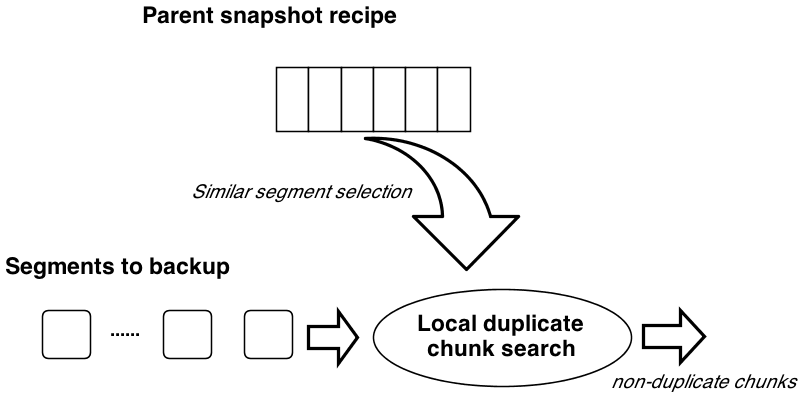
\epsfig{file=images/mh_local_dedup.png, width=3in}
  \caption{Similarity-guided local duplicate detection}
  \label{fig:local_dedup}
\end{figure}

Since the best deduplication uses a non-uniform chunk size 
in the average of 4KB or 8KB~\cite{Jin2009},
we conduct additional local similarity guided deduplication on a snapshot by comparing
chunk fingerprints of a dirty segment 
with those in  {\em similar} segments from its parent snapshot. 
We define two segments are similar if their content signature is the same.
This segment content signature value is defined as the minimum value of all its chunk fingerprints 
computed during backup and is recorded in the snapshot metadata (called recipe). Note that this definition of
content similarity is an approximation~\cite{resemblance97}.  When processing a dirty segment,
its  similar segments can be found easily from the
parent snapshot recipe.  Then recipes of the similar segments are loaded to memory,
which contain chunk fingerprints to be compared.
To control the time cost of search, we set a limit on the number of  similar segments recipes to be fetched. 
% Then,
%given a set of data chunks within a dirty segment,  we compare  these chunk fingerprints
%with those in similar segments.  
For a 2MB segment, its segment recipe is roughly 19KB which contains about 500 chunk fingerprints and other chunk metadata,
by limiting at most 10 similar segments to search, the amount of memory for maintaining those similar segment recipes is small.
As part of our local duplicate search we also compare the current segment
against the parent segment at the same offset.

%\item 
\textbf{Global deduplication with popular chunks and replication support.}
This step accomplishes the canonical global fingerprint lookup using a popular fingerprint index.
Our key observation is that the local deduplication has removed most of the duplicates.
There are fewer deduplication opportunities across VMs while the memory and network
consumption for global comparison is more expensive.
Thus our approximation is that the global fingerprint comparison only searches for the top $k$
most popular items. This dataset is called the \textbf{PDS} (popular data set). 
We define chunk popularity as the number of unique copies of the chunk in the data-store,
i.e., the number of copies of the chunk after local deduplication.
This number can be computed periodically, e.g., on a weekly basis.
Once the popularity of all data chunks is collected, the system only maintains the top $k$
most popular chunk fingerprints (called \textbf{PDS index}) in a distributed shared memory.  
%Compared to a preliminary solution which  uses data popularity~\cite{WeiZhangIEEE}, 
%this paper provides  a more comprehensive scheme with  improved deduplication efficiency and fault tolerance, and
%analytic design guidance. 

Since $k$ is relatively small and these top $k$ chunks are shared among multiple VMs, 
we can afford to provide extra replicas for these popular chunk data to enhance the fault resilience.

%\item 
\textbf{VM-centric file system block management.}
When a chunk is not detected as a duplicate to any existing chunk, this chunk will be written
to the file system. Since the backend file system typically uses a large block size such as 64MB, each VM will 
accumulate small local chunks. We manage this accumulation process using a log-structured storage scheme built
on a distributed file system discussed in Section~\ref{sect:architecture}.
%Non-PDS chunks from the same VM are stored in one append store. 
Each file system block is either dedicated to non-PDS chunks, or PDS-chunks.
A file system block for non-PDS chunks is associated with one VM and does not contain
any PDS chunks, such that our goal of fault isolation is maintained.
In addition, storing PDS chunks separately allows special replication handling for those popular shared data. 
%%% talk something about snapshot store advantage here? %%%

%The system allows all machines conduct backups in parallel, and each machine
%conducts the backup of one VM at a time, and thus only requires a write buffer for one VM.
%\end{itemize}

\begin{figure}
\centering
%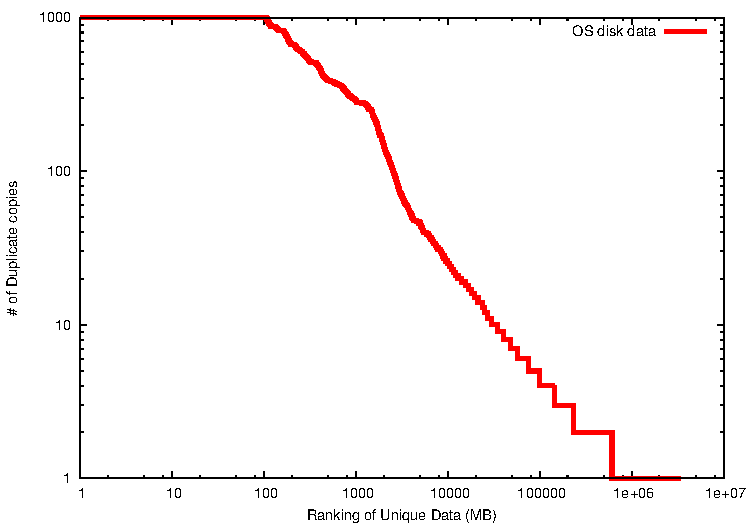
\epsfig{file=log-log.disk,width=3in}
%source ../vm_snapshot_sim/images/log-log.disk.eps
 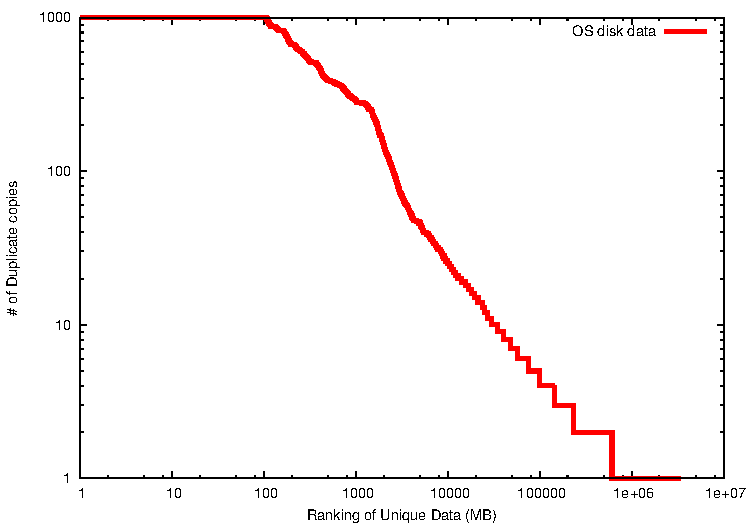
\includegraphics[width=3in]{figures/log-log-disk}
\caption{Duplicate frequency versus  chunk ranking in a log scale after local deduplication.}
\label{fig:Datazipf}
\end{figure}


% {\it [Need to find a place to put these numbers in: Total number of chunks 
% in 350 snapshots: 1,546,635,485. 
% Total number of chunks after localized dedup: 283,121,924. Total number of unique chunks: 87,692,682.]}
\subsection{Impact on deduplication efficiency}
Choosing the value $k$ for the most popular chunks affects the deduplication efficiency.
We analyze this impact based on the characteristics  of the VM snapshot traces
studied from  application datasets.
A previous study shows that the popularity of data chunks after local deduplication follows 
a Zipf-like distribution\cite{Breslau1999a} and its
exponent $\alpha$ is ranged between 0.65  and  0.7~\cite{WeiZhangIEEE}. 
Figure~\ref{fig:Datazipf} illustrates the Zipf-like distribution of chunk popularity.
The parameters we will use in our analysis below are defined in
Table~\ref{tab:symbol}. 

\begin{table}[htbp]
\centering
\begin{tabular}{|p{1.25cm}|p{5.5cm}|}
\hline
$k$ &  the number of top most popular chunks selected for deduplication\\ 
\hline
$c$ &  the total amount of data chunks in a cluster of VMs\\ 
\hline
$c_u$ &  the total amount of unique fingerprints after perfect  deduplication\\
\hline
$f_i$ &  the frequency for the $i$th most popular fingerprint\\
\hline
$\delta$ &  the percentage of duplicates detected in local deduplication\\
\hline
$\sigma$ & =$\frac{k}{c_u}$ which is  the percentage of unique data  belonging to  PDS\\
\hline
$p$ & the number of machines in the cluster\\
% \hline
% $V$ & the average number of VMs hosted on each machine\\
\hline
$E_c, E_o$ & deduplication efficiency of VC and VO \\
%\hline
%$D$ & the amount of unique data on each machine\\
%\hline
%$C$ & the average data chunk size. Our setting is  4K.\\
%\hline
%$s$ & the average size of file system blocks in the distributed file system. The default is  64MB.\\
%\hline
%$m$ & memory size on each node used by VC\\ 
%\hline
%$E$ & the size of an popular data index entry\\
\hline
$N_1$ & the average number  of non-PDS FSBs blocks in a VM for VC\\
\hline
$N_2$ & the average number  of PDS FSBs in a VM for VC\\
\hline
$N_o$ & the average number  of FSBs  in a VM for VO\\
\hline
A(r) & the availability of an FSB  with replication degree $r$\\
\hline
\end{tabular}
\caption{Modeling  parameters}
\label{tab:symbol}
\end{table}


%Table~\ref{tab:symbol} defines paramters $c$, $c_u$, $f_i$, and $\delta$ used below.
%let $c$ be the total number of data chunks. 
%$c_u$ be the total number of fingerprints 
%in the global index after complete deduplication, and
%$f_i$ be the frequency for the $i$th most popular fingerprint. 
By Zipf-like distribution, $f_i = {f_1}/{i^\alpha}.$
The total number of chunks in our backup storage which
has local duplicates excluded is $c (1-\delta)$, this can be represented
as the sum of each unique fingerprint times its frequency:
%Since $ \sum_{i=1}^{c_u}f_i = c (1-\delta)$,
\[
f_1 \sum_{i=1}^{c_u}\frac{1}{i^\alpha} = c (1-\delta).
\]
Given $\alpha <1$, $f_1$ can be approximated with integration:
\begin{equation}
f_1=\frac{c(1-\alpha)(1-\delta)}{c_u^{1-\alpha}}.
\end{equation}

Thus putting the $k$ most popular fingerprints into PDS index can remove the following number of chunks during global 
deduplication:
\[
f_1 \sum_{i=1}^{k}\frac{1}{i^\alpha} \approx  
f_1 \int_{1}^{k}\frac{1}{x^\alpha} dx  \approx  f_1\frac{  k^{1-\alpha}} {1-\alpha}
=c(1-\delta) \sigma^{1-\alpha}.
\]

Deduplication efficiency of the VC approach using top $k$ popular chunks
is the percentage of duplicates that can be detected:  
\begin{equation}
\label{eq:dedupeff}
%\begin{split}
%e_k &= 
E_c=\frac{ c\delta + c(1-\delta) \sigma^{1-\alpha}}
{c  - c_u }.\\
%\end{split}
\end{equation}

% After the global deduplication, the number of remaining chunks is:
% \[
% c-E(c-c_u)
% \] 

We store the PDS index using a distributed shared memory hash table such as Memcached
and allocate a fixed percentage of memory space per physical machine for top $k$ popular items.
As the number of physical machines ($p$) increases,
the entire cloud cluster can host more VMs; however,  ratio $\sigma$ which is $k/c_u$ remains
a constant because each physical machine on average still hosts a fixed constant number of 
VMs. Then the overall deduplication efficiency of VC defined in Formula~\ref{eq:dedupeff}
remains constant.
Thus the deduplication efficiency is stable  as $p$ increases as long as $\sigma$  is a constant.


\begin{figure}[htbp]
  \centering
    \begin{tikzpicture}
            \begin{axis}[
            %title={PDS Coverage},
            width=\linewidth,
            height=0.6\linewidth,
            cycle multi list={
                mline\nextlist
                [3 of]mmark*\nextlist
            },
            %cycle list name=mcolor,
            xlabel={Total num. chunks stored (in billions)},
            ylabel={PDS Coverage (\%)},
            %extra y ticks={4.5,5.5,6.5} %to add extra ticks
            mark options=solid,
            %legend pos=outer north east,
            legend columns=2,
            legend style={
                at={(0.5,-0.30)},
            anchor=north},
            ]
            \addplot table[x expr=\thisrow{InputChunks}/1000000000,y=A1] {figures/cds_coverage.txt};
            \addplot table[x expr=\thisrow{InputChunks}/1000000000,y=A2] {figures/cds_coverage.txt};
            \addplot table[x expr=\thisrow{InputChunks}/1000000000,y=A4] {figures/cds_coverage.txt};
            \addplot table[x expr=\thisrow{InputChunks}/1000000000,y=T1] {figures/cds_coverage.txt};
            \addplot table[x expr=\thisrow{InputChunks}/1000000000,y=T2] {figures/cds_coverage.txt};
            \addplot table[x expr=\thisrow{InputChunks}/1000000000,y=T4] {figures/cds_coverage.txt};
            \legend{Measured ($\sigma=1\%$),Measured ($\sigma=2\%$),Measured ($\sigma=4\%$),Predicted ($\sigma=1\%$),Predicted ($\sigma=2\%$),Predicted ($\sigma=4\%$)};
            \end{axis}
    \end{tikzpicture}
  \caption{Predicted vs. actual PDS coverage as data size increases.}
  \label{fig:cds-coverage}
\end{figure}
Ratio $\sigma^{1-\alpha}$ represents the percentage of the remaining
chunks detected as duplicates in global deduplication due to PDS.
We call this PDS coverage.
Figure~\ref{fig:cds-coverage} shows predicted PDS coverage using $\sigma^{1-\alpha}$ when $\alpha$ is fixed at
0.65 and measured PDS coverage in our test dataset.
$\sigma=2\%$ represents memory usage of approximately 100MB memory per machine for the PDS.
While the predicted value remains flat, measured PDS coverage increases as more VMs are involved.
This is because the actual $\alpha$ value increases with the data size.
%Then  PDS coverage PDS increases as more VMs are involved.

\subsection{ Impact on Fault Isolation}
 
\begin{figure}
    \centering
    \subfigure[Sharing of file system blocks under VC]
    {
        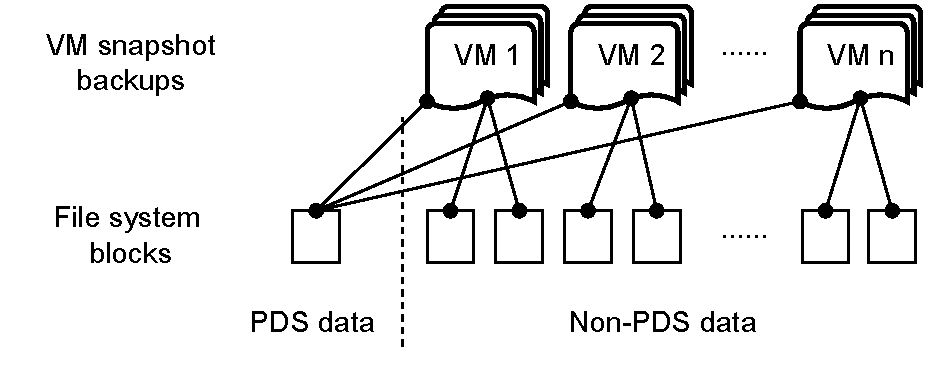
\includegraphics[width=3in]{images/share_vc}
        \label{fig:share_vc}
    }
    \\
    \subfigure[Sharing of file system blocks under VO]
    {
        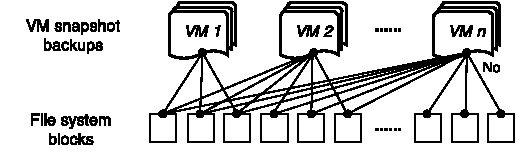
\includegraphics[width=3in]{images/share_vo}
        \label{fig:share_vo}
    }
    \caption{Bipartite association of VMs and file system blocks under (a) VC and (b) VO. }
    \label{fig:share}
\end{figure}

The replication degree of the backup storage 
is $r$ for regular file system blocks and $r=3$ is a typical setting in distributed
file systems~\cite{googlefs03,hdfs10}.
Since $\sigma$ is small (e.g.  2\% in our experiments),  
the impact of replication on storage increase is very small even 
when choosing  $r_c/r$ ratio as 2 or 3. 


%In the VC approach, a special replication degree $r_c$ is used for PDS data where $r_c>r$. 
%The storage cost for VO with full deduplication is $c_u *r$ and for VC, it is
%$ k*r_c  + (c-E(c-c_u))*r$. Thus The storage cost ratio of $VC$ over $VO$ is 
%\[
%\sigma \frac{r_c}{r} + \frac{c-e(c-c_u)}{c_u}.
%\]
%Since $\sigma$ is small (it is 2\% in our experiments),  
%term $\sigma \frac{r_c}{r}$ is small in the above expression.  
%Thus the impact on storage increase is very small even when we choose a large $r_c/r$ ratio. 
%For example, $r_c/r=2$ or 3. 

Now we  assess  the impact of losing $d$ machines 
to the VC and VO approaches.  
A large $r_c/r$ ratio can have a positive impact on full availability of VM snapshot blocks.
We use an FSB rather than a deduplication
data chunk as our unit of failure because the DFS keeps
file system blocks as its base unit of storage.
To compute the full availability of all snapshots of a VM, we derive
the probability of losing a snapshot FSB of a VM by
estimating the number of file system blocks per VM in each approach.
As illustrated in Figure~\ref{fig:share},
we build a bipartite graph representing the association from unique file system blocks
to their corresponding VMs in each approach. An association edge is  drawn  from an FSB to a VM 
if this block is used by the VM. 

For VC, each VM has an average number of $N_1$ non-PDS FSBs
and  has  an average of  $N_2$ PDS FSBs. 
Each non-PDS FSB is associated with one VM
 and  we denote that PDS FSBs are
shared by an average of $V_c$ VMs. Let $s$ be the average number of chunks per file system block, 
$V$ be the average number of VMs hosted on each machine. Then, 
\[
V pN_1 s  \approx c-E_c(c-c_u) - c_u\sigma\; \mbox{ and } \; 
V pN_2 s  \approx c_u \sigma V_c.
\]

For VO, each VM has an average of $N_o$ FSBs
and let $V_o$ be the average number of VMs shared by each FSB.
\[
V pN_o s  = (c- E_o(c-c_u) ) V_o.
\]

Since each FSB (with default size $64MB$) contains many chunks (on average 4KB),
each FSB contains the hot low-level chunks shared by many VMs, and it also contains
rare chunks which are not shared.  Since $c>> c_u$, from the above equations:
\[
\frac{N_1}{N_o} \approx  \frac{1-E_o}{(1-E_c) V_o}.
\] 
When $E_c$ is close to $E_o$ as demonstrated in Section~\ref{sect:evaldedup}, $N_1$ is 
much smaller than $N_o$. 
%When there is a failure in FSBs with replication degree $r$
%and there is no failure for PDS data with more replicas,   a VM in
%the VC approach has a much lower chance to lose a snapshot than VO. 
%Figure~\ref{fig:fsb-links} shows the average number of VMs sharing each file block from
%our test dataset.
%For VC, we only show
%the sharing degree of  PDS-oriented file blocs  because non-PDS blocks always belong to
%one VM.
%Figure~\ref{fig:fsb-links} shows the average number of VMs sharing each file block from our test data.
Figure~\ref{fig:vm-links} shows the average number of file system blocks for each VM in VC and in VO
and  $N_1$ is indeed  much smaller than $N_o$ in our tested dataset.  
%In fact, $N_1 +N_2 < N_o$. 
%This is likely because the PDS FSBs tightly pack data used by many VMs, 
%which decreases the overall number of FSBs required to backup a VM.
%Note that  if  the backup for multiple VMs were conducted concurrently, there could be many more
%VMs sharing each file block on average in VO. 

%Therefore, even when there is a loss of a PDS block, the VC approach tolerates the fault better.

\comments{
\begin{figure}[htbp]
  \centering
	\begin{tikzpicture}
		\begin{axis}[
                width=\linewidth,
                height=0.6\linewidth,
		%title={VO FSB links},
		xlabel={Number of VMs},
		ylabel={Avg. Num. VMs sharing FSB},
                cycle list name=mline,
                xmin=0,
                ymin=0,
                xmax=106,
		%extra y ticks={4.5,5.5,6.5} %to show extra ticks
		legend pos=north west
		]
                \addplot table[x=VMs,y=FSBLinks] {figures/vo_fsb_links_105.txt};
		\addplot table[x=VMs,y=cdslinks] {figures/cds_links_105.txt};
                \legend{VO, PDS in VC};
		\end{axis}
	\end{tikzpicture}
  \caption{Measured average number of VMs sharing a 64MB FSB in VO and in VC.}
  \label{fig:fsb-links}
\end{figure}

}

\begin{figure}[htbp]
  \centering
	\begin{tikzpicture}
		\begin{axis}[
		%title={VO VM links},
                width=\linewidth,
                height=0.6\linewidth,
		xlabel={Number of VMs},
		ylabel={Avg. Num. FSBs used by VM},
                xmin=0,
                ymin=0,
                xmax=106,
		%extra y ticks={4.5,5.5,6.5} %to show extra ticks
		%legend pos=north east,
                legend style={
                    at={(1,0.825)},
                    anchor=north east
                },
                %legend columns=3
		]
                \addplot[blue,mark=none] table[x=VMs,y=N_O] {figures/vm_links_all.txt};
                %\addplot[red,dotted,mark=none] table[x=VMs,y expr=\thisrow{N_1}+\thisrow{N_2}] {figures/vm_links_all.txt};
                \addplot[red,dashdotted] table[x=VMs,y=N_1] {figures/vm_links_all.txt};
                \addplot[red,densely dashed,mark=none] table[x=VMs,y=N_2] {figures/vm_links_all.txt};
                \legend{$N_o$,
                    %$N_1+N_2$,
                    $N_1$,
                    $N_2$};
		\end{axis}
	\end{tikzpicture}
  \caption{Measured average number of 64MB FSBs used by a single VM. For VC both the number of PDS and Non-PDS FSBs used are shown.}
  \label{fig:vm-links}
\end{figure}

The full snapshot availability of a VM is estimated as follows with parameters $N_1$ and
 $N_2$ for VC and $N_o$ for VO.
Given normal data replication degree $r$, PDS data replication degree $r_c$, 
the availability of a file system block is the probability that  
all of its replicas do not appear in any group of $d$ failed machines among the total of $p$ machines. 
Namely, we define it as
\[
A(r) = 1-\binom{d}{r}/ \binom{p}{r}. 
\]
Then the availability of one VM's snapshot data under VO approach is the probability that
 all its FSBs are unaffected during the system failure:
\begin{equation}
\label{eq:VO}
%(1-\frac{ \binom{d}{r}} { \binom{p}{r} })^{N_o}. 
A(r)^{N_o}. 
\end{equation}

For VC, there are two cases for $d$ failed machines.
\begin{itemize}
\item
When $r \le d<r_c$,  there is no PDS data loss and  
the full snapshot availability of a VM in the VC approach is 
\begin{equation}
\label{eq:VC1}
%(1-\frac{\binom{d}{r}} { \binom{p}{r} })^{N_1}.
A(r)^{N_1}.
\end{equation}
Since $N_1$ is typically much smaller than $N_o$, 
the VC approach has a higher availability of VM snapshots than VO.
In the evaluation discussed in Section~\ref{sect:evaldedup}, we have considered a worst case scenario that
every PDS FSB is shared by all VMs in the VC approach, which leads a large $N_2$ value. 
Even with that, the availability of VC snapshots is much higher than VO and we analyze  this below.

\item
When $r_c \leq d$, both non-PDS and PDS file system blocks in VC can have a loss.
The full snapshot availability of  a VM in the VC approach is
\begin{equation}
\label{eq:VC2}
% (1-\frac{ \binom{d}{r}} { \binom{p}{r} })^{N_1} 
% *
% (1-\frac{ \binom{d}{r_c}} { \binom{p}{r_c} })^{N_2}.
A(r)^{N_1} * A(r_c)^{N_2}
\end{equation}
%comparing  Formula~\ref{eq:VO} and~\ref{eq:VC}. 
\end{itemize} 
In the evaluation discussed in Section~\ref{sect:evaldedup}, we have considered a worst case scenario that
every PDS FSB is shared by all VMs in the VC approach, which leads to a large $N_2$ value. 
Even with that, the availability of VC snapshots is still much higher than VO and  
there are two reasons.  1) $N_1$ is much smaller than $N_o$ as discussed previously.
2)  $A(r) < A(r_c)$ because of  $r < r_c$.  
Table~\ref{tab:fsb-availability} lists the $A(r)$ values with
%that the availability of an individual file system block
different replication degrees, to demonstrate the gap between  $A(r)$ and  $A(r_c)$.

% $1-\frac{ \binom{d}{r}} { \binom{p}{r} } < 1-\frac{ \binom{d}{r_c}} { \binom{p}{r_c} }$

\comments{
\begin{figure}[htbp]
  \centering
    \begin{tikzpicture}
            \begin{axis}[
                width=\linewidth,
                height=0.6\linewidth,
            %title={FSB Availability},
            cycle list name=mline,
            xlabel={Number of Machines Failed},
            ylabel={Availability of Single FSB (\%)},
            %extra y ticks={99.9}, %to add extra ticks
            mark options=solid,
            legend pos=south west,
            %legend columns=2,
            %legend style={
            %    at={(0.5,-0.2)},
            %anchor=north}
            ]
            \addplot table[x=NodesFailed,y=Availability5] {figures/fsb_availability.txt};
            \addplot table[x=NodesFailed,y=Availability4] {figures/fsb_availability.txt};
            \addplot table[x=NodesFailed,y=Availability3] {figures/fsb_availability.txt};
            \legend{$R=5$,$R=4$,$R=3$};
            \end{axis}
    \end{tikzpicture}
    \caption{Availability of a file system block in a 100 machine cluster with different replication 
and failure settings.THIS PLOT WILL BE REPLACED BY TABLE}
  \label{fig:fsb-availability}
\end{figure}
}

\begin{table}
  \centering
    \footnotesize
    \tabcolsep=0.11cm
    \comments{%table data is obsolete, now uses pgfplotstable
        \begin{tabular}{|l|l|l|l|}
        \hline
        \multirow{2}{*}{Failures ($d$)}   & \multicolumn{3}{c|}{$A(r_c)\times 100\%$} \\
                                    %\cline{2-4}
                                    & $r_c=3$ & $r_c=6$ & $r_c=9$ \\
        \hline
        3 & 99.9994 & 100 & 100\\
        5 & 99.9939 & 100 & 100\\
        10 & 99.9258 & 99.9999 & 99.9999 \\
        20 & 99.2950 & 99.9967 & 99.9999 \\
        \hline
    \end{tabular}
    }
    \pgfplotstabletypeset[
        columns={NodesFailed,Availability3,Availability6,Availability9},
        columns/NodesFailed/.style={
            column name={\multirow{2}{*}{Failures ($d$)}}
        },
        columns/Availability3/.style={
            column name={\multicolumn{3}{c|}{$A(r_c) \times 100\%$}\\&$r_c=3$},
            fixed, precision=9
        },
        columns/Availability6/.style={
            column name={$r_c=6$},
            fixed, precision=9},
        columns/Availability9/.style={
            column name={$r_c=9$},
            fixed, precision=9},
        every head row/.style={
            before row={\hline},
            after row={\hline},
        },
        every last row/.style={after row=\hline},
        column type/.add={}{|},
        every first column/.style={column type/.add={|}{}},
    ]{figures/fsb_availability.txt}
    \caption{$A(r_c)$ as storage nodes fail in a 100 node cluster.}
    \label{tab:fsb-availability}
\end{table}
